\documentclass[a4paper]{article}
\usepackage{exercise}
%um nur aufgaben zu zeigen
%\usepackage[noanswer]{exercise} 
\usepackage{../images/preamble}
\usepackage{rotating}
\usetikzlibrary{decorations.pathmorphing}

\begin{document}
	\vspace*{-2cm}
	\parbox{4cm}{
\includegraphics[width=2.5cm]{../images/ROLF4.png}}
	\parbox{10.6cm}{\setstretch{2.0} \centering{ \huge \textsf{Aufgabenserie 2}}\\ Abgabe: 19. Juni \\ \vspace*{-.5cm} }
	
	

\thispagestyle{empty}
\begin{framed}
	\noindent
	\scriptsize
	Die Aufgaben sollten bis zum \textbf{19. Juni} bearbeitet werden. Die Lösungen schickt ihr entweder an \href{mailto:physikrolf@gmail.com}{physikrolf@gmail.com}, oder per Post an: Aaron Wild, Zum wilden Graben 26, 99425 Weimar.
	Jede Aufgabe hat eine bestimmte Anzahl an erreichbaren Punkten. Wie viele das sind, müsst ihr raten. Versucht, die Lösungen so genau wie möglich aufzuschreiben. Für besonders schnelle/gute/witzige Lösungen kann es Bonuspunkte geben.\\ Die aktuellen Aufgaben sowie alle alten Aufgabenserien mit Lösungen findet ihr auch auf \url{pankratius.github.io/rolf}
\end{framed}

\noindent
\begin{Exercise}[label = hypercube, origin = {Max Marienhagen, Aaron Wild}, difficulty = 5, title =  Widerstandswürfel]
Ein $n$-dimensionaler Hyperwürfel ist die Verallgemeinerung eines Würfels auf $n$ Dimensionen. Seine Konstruktion kann man sich so vorstellen, dass ein $n-1$-dimensionaler Hyperwürfel im $n$-dimensionalen Raum parallelverschoben wird, und man das daraus entstandene Volumen betrachtet.\\
Ein solcher $n$-dimensionaler Hyperwürfel hat $2^n$ Eckpunkte und $n2^{n-1}$ Seitenkanten.\\
Wir betrachten nun einen $n$-dimensionalen Hyperwürfel ($n\geq 1$), bei dem alle Seitenkanten einen Widerstand von $r$ haben. Zeige, dass der Widerstand zwischen zwei benachbarten Eckpunkten 
\begin{equation}
	R = \frac{2-2^{1-n}}{n}r = \frac{2^n-1}{n2^{n-1}}r
\end{equation}
beträgt. Überlege dir an einem $n$ deiner Wahl, dass das Ergebnis dort sinnvoll ist.
\end{Exercise}
\begin{Answer}[ref = hypercube]
	Diese Aufgabe kann sehr schön einfach und elegant mithilfe des Superpositionsprinzips gelöst werden.\\
	Wir betrachten dazu zwei benachbarte Ecken des Würfels - nennen wir sie $A$ und $B$. Nun schauen wir uns zwei Fälle an:
	\begin{enumerate}
	\item Ein Strom $I$ wird in Ecke $A$ eingespeist. Die Spannungen an allen Ecken des Hyperwürfels werden so eingestellt, 	dass an jeder Ecke außer $A$ derselbe Strom aus dem Würfel fließt. Da es $2^n$ Ecken gibt und der ausfließende Strom 		insgesamt wieder $I$ sein muss, fließt also an jeder Ecke außer $A$ der Strom $\frac{I}{2^n-1}$ aus dem Würfel.\\
	Im $n$-dimensionalen Hyperwürfel hat jede Ecke $n$ direkt benachbarte Ecken. (Weil der Hyperwürfel durch $n-1$ 			Paralleverschiebungen aus dem eindimensionalen Hyperwürfel entsteht und bei jeder Parallelverschiebung eine benachbarte 	Ecke hinzukommt.) Das heißt, dass von der Ecke $A$ $n$ Widerstände abgehen. Durch jeden dieser Widerstände fließt aus 		Symmetriegründen ein Strom $\frac{I}{n}$ von $A$ weg.
	\item An jeder Ecke außer $B$ wird ein Strom $\frac{I}{2^n-1}$ in den Hyperwürfel eingespeist. Bei Ecke $B$ fließt ein 		Strom $I$ aus dem Würfel heraus. Aus Symmetriegründen fließt durch die $n$ direkt an $B$ anliegenden Widerstände ein Strom 	   von jeweils $\frac{I}{n}$.  
	\end{enumerate}
	Jetzt betrachten wir die Superposition beider Fälle. Das heißt, wir addieren für jede Ecke das dort anliegende Potenzial im 	    ersten und zweiten Fall. Für jeden Widerstand addieren wir (vorzeichenbehaftet) die im ersten und zweiten Fall 		durchfließenden Ströme\footnote{Das darf man machen, weil die Ohmschen Gesetze linear sind.}.\\
	Schauen wir uns zunächst alle Ecken, außer $A$ und $B$ an. Im ersten Fall verlässt ein Strom $\frac{I}{2^n-1}$ aus dem 		Hyperwürfel heraus. Im zweiten Fall fließt an jeder dieser Ecken genau derselbe Strom in den Hyperwürfel hinein. Das heißt, 	    dass in der Superposition an all diesen Ecken kein Strom in den Würfel rein oder aus ihm raus fließt.\\
	Nun schauen wir uns Ecke $A$ an: Im ersten Fall fließt der Strom $I$ dort in den Würfel, im zweiten Fall der Strom 		$\frac{I}{2^n-1}$. In der Superposition fließt also an der Ecke $A$ ein Strom von $I+\frac{I}{2^n-1}$    	       in den Hyperwürfel herein. Aus Ecke $B$ fließt nach einer ganz ähnlichen Argumentation genau derselbe Strom heraus (muss ja auch so sein, weil wir gerade gesehen haben, dass bei allen anderen Ecken kein Strom rein- oder rausgeht). Dieser Strom ist also auch der Gesamtstrom, der von $A$ nach $B$ fließt.\\
	Als nächstes sehen wir uns den Widerstand zwischen $A$ und $B$ an. Im ersten und im zweiten Fall fließt ein Strom von $\frac{I}{n}$ durch ihn. In beiden Fälle geht der Strom in die gleiche Richtung (von $A$ zu $B$). Das heißt, in der Superposition fließt ein Strom von $2\frac{I}{n}$ durch diesen Widerstand von $A$ zu $B$. Nach der Definition des Widerstands\footnote{$R=\frac{U}{I}$. Aber das solltet ihr eigentlich auch selber wissen...}, ist die an diesem Widerstand abfallende Spannung deshalb $U=r\cdot 2\frac{I}{n}$. Diese Spannung ist also gleich der Potenzialdifferenz zwischen $A$ und $B$. Jetzt können wir die Definition des Widerstandes gleich nochmal benutzen! Denn nun kennen wir den gesamten Strom, der von $A$ nach $B$ fließt ($I+\frac{I}{2^n-1}$) und die Spannungsdifferenz zwischen $A$ und $B$ ($r\cdot 2\frac{I}{n}$). Dann gilt also:
	\begin{equation*}
	R = \frac{r\cdot 2\frac{I}{n}}{I+\frac{I}{2^n-1}} = \frac{r\cdot 2\frac{I}{n}}{I+\frac{I}{2^n-1}} \cdot \frac{2^n-1}{2^n-1} = \frac{(2^n-1)\cdot \frac{2r}{n}}{2^n-1+1} = \frac{2(2^n-1)}{n \cdot 2^n}r = \frac{2(2^n-1)}{n \cdot 2 \cdot 2^{n-1}}r = \frac{2^n-1}{n2^{n-1}}r
	\end{equation*}
	Das ist das gesuchte Ergebnis.\\
	Übrigens kann man solche Superpositionstricks sehr oft bei allen möglichen Aufgaben mit Widerstandsnetzen oder Ähnlichem anwenden und sie so enorm vereinfachen.  
	Anders geht es über eine widerliche Sache - Das macht Aaron.
\end{Answer}

\begin{Exercise}[label=heate, origin = {US IPhO Auswahlwettbewerb, Halbfinale 2013}, title = Wärmetauscher,difficulty = 4]
Die durch Wärmeleitung übertragene Wärmeleistung zwischen zwei parallelen Wänden kann näherungsweise durch die Gleichung 
\begin{equation}\label{he:fg}
	P = \lambda A \frac{T_a-T_b}{d}
\end{equation}
beschrieben werden. Dabei ist $A$ die Fläche, durch die Wärme strömt, $d$ der Abstand zwischen den beiden Wänden und $\lambda$ eine Konstante, die vom Material zwischen den beiden Wänden abhängt (die sog. Wärmeleitfähigkeit). $T_a$ ist die Temperatur der wärmeren Wandoberfläche und $T_b$ die der kälteren Wandoberfläche.\\
Ein Wärmetauscher ist ein Gerät, dass Wärme von einer warmen Flüssigkeit zu einer kälteren Flüssigkeit überträgt (Abb. \ref{fig:heate}).
Dabei fließt warme Flüssigkeit (rot) mit einer Geschwindigkeit $v$ von rechts nach links, und kalte Flüssigkeit (blau) mit einer Geschwindigkeit von $v$ von links nach rechts. Die Dichte der Flüssigkeiten ist $\rho$ und die Wärmekapazität $c$. Beide befinden sich in Röhren der Höhe $h$ ($h$ ist sehr klein).  Die beiden Flüßigkeiten sind durch eine Metallwand (grau) der Dicke $d$ mit der Wärmeleitfähigkeit $\lambda$ getrennt. \\
Die Temperaturdifferenz zwischen der einfließenden warmen Flüssigkeit und der einfließenden kalten Flüssigkeit beträgt $\Delta T_e$. \\
Bestimme die Temperaturdifferenz zwischen der abgekühlten, ausfließenden warmen Flüssigkeit und der aufgewärmten, ausfließenden kalten Flüßigkeit, $\Delta T_a$. Nimm dafür an, dass die Temperaturdifferenz $\Delta T$ zwischen warmer und kalter Flüssigkeit entlang der Wand konstant bleibt.

\end{Exercise}
\begin{figure}[h]
	\centering
	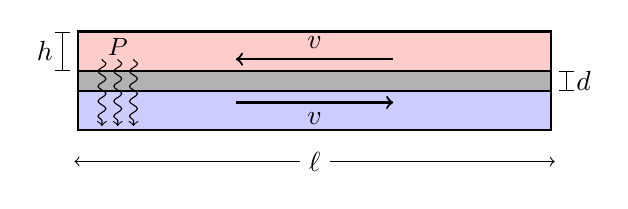
\begin{tikzpicture}

\filldraw[thick, draw = black, fill = red!20!white] (-3,-0.25)rectangle (3,.25);
\filldraw[thick, draw = black, fill= black!30!white] (-3,-0.5)rectangle (3,-.25);
\filldraw[thick,draw= black, fill=blue!20!white] (-3,-1)rectangle(3,-.5);

\draw[|-|] (3.2,-.25)--(3.2,-.5) node [midway, right] {$d$};

\draw[->,thick] (-1,-.65) -- (1,-.65) node[midway, below] {$v$};
\draw[<-,thick] (-1,-.1)--(1,-.1) node[midway, above]{$v$};
\draw[->,decorate,decoration={snake, amplitude = 0.5mm, segment length = 1.9mm}] (-2.5,-0.1) -- (-2.5,-.95);
\draw[->,decorate,decoration={snake, amplitude = 0.5mm, segment length = 1.9mm}] (-2.7,-0.1) -- (-2.7,-.95);
\draw[->,decorate,decoration={snake, amplitude = 0.5mm, segment length = 1.9mm}] (-2.3,-0.1) -- (-2.3,-.95);
\node at (-2.5,0.05) {\small $P$};
\draw[|-|] (-3.2,.25)--(-3.2,-.25) node[midway, left]{$h$};
\draw[<->] (-3.05,-1.4) -- (3.05,-1.4) node[midway, fill = white] {$\ell$};
\end{tikzpicture}
	\caption{Ein Wärmetauscher}
	\label{fig:heate}
\end{figure}
\begin{Answer}[ref= heate]
	Die warme (rote) Flüssigkeit strömt mit einer Temperatur $T_{w,e}$ in den Wärmetauscher und verlässt ihn mit einer Temperatur $T_{w,a}$. Diese Temperaturänderung  $\Delta T_w$ kommt durch den Wärmeaustausch mit der Leistung $P$ aus \eqref{he:fg}. 
	Diese ist definiert als die Wärmezufuhr pro gegebener Zeiteinheit, also $P = \frac{Q}{t}$. Die Zeit $t$, in der hier die warme Flüssigkeit Wärme abgibt, ist genau die Zeit, die gebraucht wird, um die Röhre des Wärmetauschers zu durchlaufen, also $ t = \frac{\ell}{v}$. In dieser Zeit fließt eine Masse von $m = \rho V = \rho A h$ durch den Wärmetauscher, wobei $A$ genau die Fläche ist, über die die Wärmeübertragung stattfindet. Die Temperaturänderung $\Delta T_w$ kann also über die abgegebene Leistung berechnet werden zu
	\begin{equation}\label{he:tloss}
		P = -\frac{Q}{t} = \frac{m c \Delta T_w}{t} \Rightarrow \Delta T_w =- \frac{Pt}{mc} \overset{\eqref{he:fg}}{=} \underbrace{\frac{\lambda A \Delta T }{d}}_{=P}\cdot \underbrace{\frac{\ell}{v}}_{= t}\cdot \underbrace{\frac{1}{\rho c A h}}_{=\frac{1}{mc}} = -\frac{\lambda \Delta T\ell}{dv\rho c h}.
	\end{equation}
	Da wir die Temperatur der ausfließenden warmen Flüssigkeit $T_{w,a}$ auch durch die der einfließenden kalten Flüssigkeit $T_{k,e}$ und die (konstante) Temperaturdifferenz zwischen den beiden Wänden $\Delta T$ ausdrücken können, ist
	\begin{equation}\label{he:dtr}
		\Delta T_{w} = T_{w,a} - T_{w,e} = T_{k,e}+\Delta T - T_{w,e} = \Delta T - \Delta T_e,
	\end{equation}
	wobei $\Delta T_e$ die Temperaturdifferenz der einfließenden Flüssigkeiten ist. 
	Wir können \eqref{he:tloss} und \eqref{he:dtr} gleichsetzten, und so die Temperaturdifferenz zwischen den Wänden bestimmen
	\begin{equation}\label{he:tdiffwall}
	-\frac{\lambda \Delta T\ell}{dv\rho c h} = \Delta T - \Delta T_e \Rightarrow \Delta T \left(1+\frac{\lambda \ell}{dv\rho c h}\right) = \Delta T_e\Rightarrow \Delta T = \Delta T_e \left(1+\frac{\lambda \ell}{dv\rho c h}\right)^{-1}.
	\end{equation}
	Durch $\Delta T$ können wir jetzt die gesuchte Temperaturdifferenz zwischen den ausfließenden Flüssigkeiten $\Delta T_a$ finden. Es ist 
	\begin{equation}
	\boxed{
		\Delta T_a = T_{w,a} - T_{k,a} = T_{k,e} + \Delta T - \left(T_{w,e}-\Delta T\right) = 2\Delta T - \Delta T_{e} =\Delta T_e\left( \frac{2}{1+\frac{\lambda \ell}{dv\rho c h}}-1\right).}
	\end{equation}
\end{Answer}
\begin{minipage}[b]{0.8\textwidth}
\noindent
\begin{Exercise}[label = can, title = {Büchse}, origin = {nach 3. Runde IPhO, 2011},difficulty = 1]
	Bestimme die Position des Schwerpunkts $h_s$ einer gefüllten zylinderförmigen Büchse in Abhängigkeit der Füllhöhe $h_f$ und der relevanten Parameter. Nimm dafür an, dass die Büchse eine gleichmäßige Massenverteilung hat. 
\end{Exercise}
\end{minipage}
\begin{minipage}[b]{0.2\textwidth}
\centering
\begin{tikzpicture}
\draw (-0.5,1)--(-0.5,0)--(0.5,0)--(0.5,1);
\fill[pattern = north east lines] (-0.5,0.6)--(-0.5,0)--(0.5,0)--(0.5,0.6);
\filldraw[black] (0,0.3) circle (2pt);
\draw[<->] (0.7,0) -- (0.7,0.3) node[midway, right]{$h_s$} ;
\draw[<->] (-0.7,0) -- (-0.7,0.6) node[midway, left]{$h_f$};

\end{tikzpicture}
\end{minipage}
\begin{Answer}[ref = can]
	Weil die Büchse eine gleichmäßige Massenverteilung hat, und wir auch annehmen können, dass die Flüssigkeit eine gleichmäßige Dichte hat, muss das System rotationssymetrisch um die senkrechte Achse durch den Deckel und den Boden sein. Das heißt aber nichts anderes, als das eine Drehung der Büchse um diese Achse keine messbaren Unterschiede hervorbringen kann, weshalb der Schwerpunkt in auf dieser Achse liegen muss. Wäre das nämlich nicht so, gäbe es eine Möglichkeit, festzustellen, wie die Büchse um diese Achse gedreht wurden ist, welche es aber wegen der Rotationssymetrie nicht geben darf.\\
	Die Höhe des Schwerpunkts kann man nun am Einfachsten über die Definitionsgleichung bestimmen. Dafür stellen wir uns das System zusammengesetzt aus der Flüssigkeit und der Büchse vor. Der Schwerpunkt der Büchse liegt bei $h_{Sp,b} = \frac{h_b}{2}$, wobei $h_b$ die Höhe der Büchse ist, und der der Flüssigkeit liegt bei $h_{Sp,f}=\frac{h_f}{2}$. Die Höhe $h$ des Gesamtschwerpunkts (relativ zum Boden der Büchse) ist gegeben durch
	\begin{equation}\label{can:spdef}
		h = \frac{m_{b}h_{Sp,b}+m_{f}h_{Sp,f}}{m_{b}+m_{f}},
	\end{equation}
	wobei $m_b = \rho_b h_b$ die Masse der Büchse ist, und $m_f = \rho_f h_f$ die Masse der Flüßigkeit. Setzt man diese beiden Ausdrücke in \eqref{can:spdef} ein, so erhält man
\end{Answer}





%
%\newpage
%\begin{turn}{270}
%\definecolor{qqttcc}{rgb}{0.,0.2,0.8}
\definecolor{ffqqqq}{rgb}{1.,0.,0.}
\definecolor{ffqqtt}{rgb}{1.,0.,0.2}
\definecolor{cqcqcq}{rgb}{0.7529411764705882,0.7529411764705882,0.7529411764705882}
\begin{tikzpicture}[line cap=round,line join=round,>=triangle 45,x=0.75cm,y=0.75cm]
\draw [color=cqcqcq,, xstep=1.5cm,ystep=1.5cm] (-8.5,0.6) grid (23.,20.);
\clip(-8.5,0.6) rectangle (23.,20.);
\draw (-5.588239388018447,9.518801182219294) node[anchor=north west] {$S$};
\begin{scriptsize}
\draw [fill=black] (-5.65741495087795,9.439855831290508) circle (2.5pt);
\draw [fill=ffqqtt] (1.9550099267845686,14.114279339778834) circle (2.0pt);
\draw [fill=ffqqqq] (17.86598524604952,10.425615052655644) circle (2.0pt);
\draw [fill=qqttcc] (2.6268608640983873,14.364446314147006) circle (2.0pt);
\draw [fill=qqttcc] (18.279983363360785,9.990865906507295) circle (2.0pt);
\end{scriptsize}
\end{tikzpicture}
%\end{turn}



\end{document}
